\chapter[PAM Generation and Demodulation]{PAM Generation and Demodulation}

\section*{Aim}
To set-up and implement circuits to carry out pulse amplitude modulation. To design demodulationg circuits to detect the message from pulse amplitude modulated wave.
\section*{Theory}
Pulse amplitude modulation is a kind of modulation technique in which analog message signal is sampled at constant frequency - \emph{carrier frequency}. A pulse of specified duration is used to sample the message signal. When the pulse is on, the message is sampled and when it is off no message is sampled. This is a basic step in the digitization of analog message signals. The circuits to be implemented in this experiment does a kind of natural sampling.\footnote{For more on natural sampling, refer Digital Transmission \cite{Tomasi}}.

Waveforms showing pulse carriers whose amplitude is modulated buy meg=ssage is shown in Figure \ref{PAMmod}.
\begin{figure}[h]
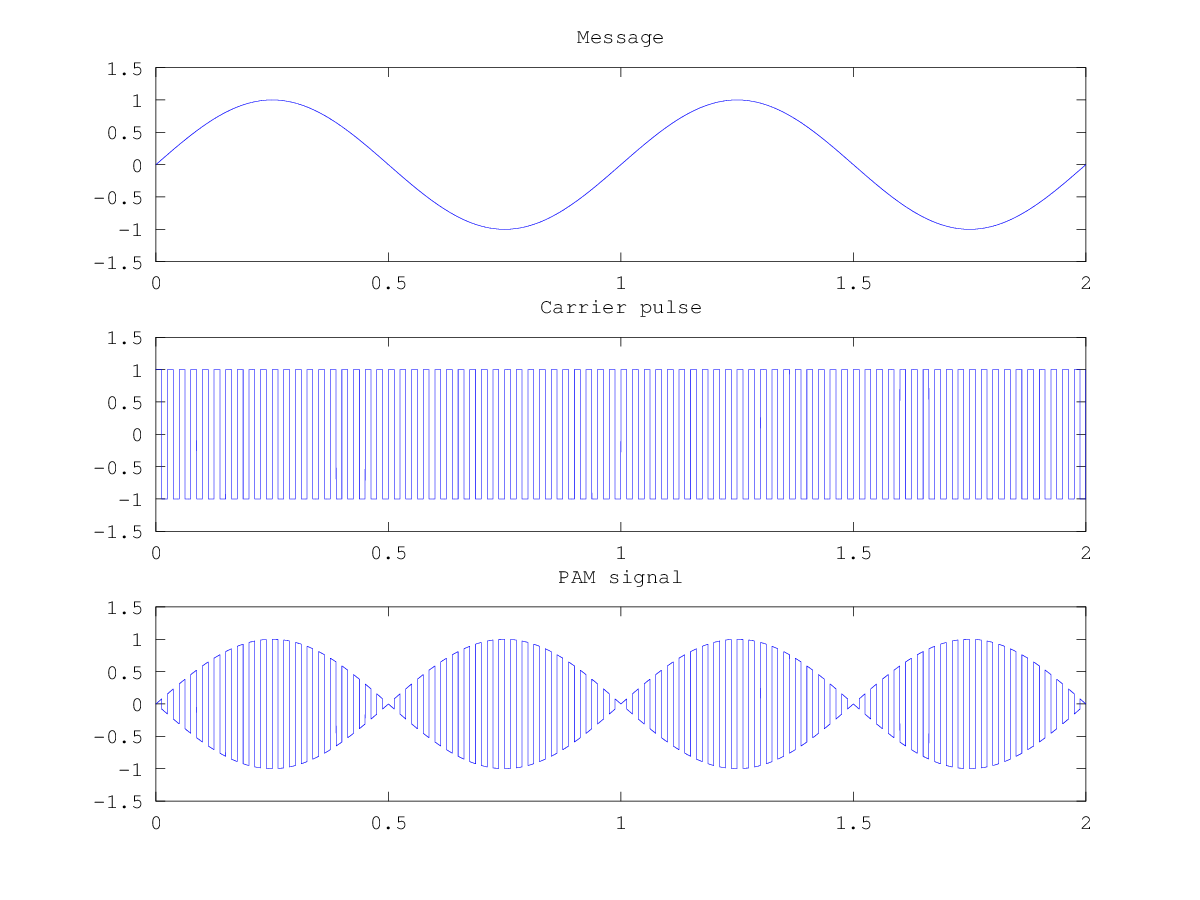
\includegraphics[width=\textwidth]{pam.png}
\caption{PAM modulation}
\label{PAMmod}
\end{figure}
\section*{Design}
\subsection*{Using transistor as a switch}
\subsection*{Using CMOS switching IC CD4016}

\section*{Circuit Diagram}
\subsection*{Using transistor as a switch}
\subsection*{Using CMOS switching IC CD4016}

\section*{Procedure}
\section*{Observation}
\section*{Result}